\documentclass[12pt, oneside]{article}
\usepackage[letterpaper]{geometry}
\usepackage{Logemann}
\usepackage{SetTheory}
\usepackage{Sum}
\usepackage{Product}
\usepackage{listings}
\usepackage{tikz}
\usetikzlibrary{shapes.geometric}
\usetikzlibrary{arrows}
\tikzstyle{vertex_style}=[circle, draw, inner sep=2pt, align=center]
%\usepackage{jlcode}

\begin{document}
\noindent \textbf{\Large{Caleb Logemann \\
AERE 504 Intelligent Air Systems \\
Final Take-Home Exam
}}

\begin{enumerate}
  \item[\#1] % Done
    What is the size of the state space?

    The state space is the product of the number of options of $r$, $h$ and $t$.
    So the size of the state space is $2 \times 21 \times 11 = 462$.

  \item[\#2] % Done
    What is the size of the observation space?

    After each action we know that $t$ decreases by one, and we can't directly
    observe if aircraft $B$ is responsive or not.
    We can only observe the new $h$.
    So the size of the observation space is $21$.

  \item[\#3] % Done
    What is the dimensionality of our belief state?

    The only unobservable part of the state space is the responsiveness $r$ of
    aircraft $B$, so the dimensionality of the belief space is 1.
    The belief state will be a single parameter $p$ which will represent the
    probability that $r = 0$, and thus $1 - p$ is the probability that $r = 1$.

  \item[\#4] % Done
    Assume our initial belief is uniform over all states with $t = 10$.
    After the first observation, how many components of the belief vector will
    be non-zero?

    After the first observation we know $h$ and $t$ exactly, so the only
    unknown is $r$.
    If we started with an uniform belief that would mean that intially we assign
    each possibility probability $0.5$.
    One observation won't change this probability to zero.
    This means that the only component of the belief vector will be non-zero.

  \item[\#5] % Done
    Suppose we have a belief $b$ that assigns probability $1$ to state
    $\br{1, 10, 1}^T$; what is $Q^*(b, a_{+1})$ (assume $\lambda = -0.5)$?
    Provide an exact numerical value and explain.

    From this state and taking this action there are two possible future states
    either $\br{1, 10, 0}^T$ with probability $.75$ or $\br{1, 9, 0}^T$ with
    probability $.25$.
    In either case the aircraft will not collide and the best action to take
    is $a_0$, so we know that
    \[
      U(\br{1, 10, 0}^T) = U(\br{1, 9, 0}^T) = 0
    \]
    Thus we can compute $Q^*(b, a_{+1})$ as
    \begin{align*}
      Q^*(b, a_{+1}) &= R(s, a) + \sum{s'}{}{T(s'|s, a)U(s')} \\
      &= R(\br{1, 10, 1}^T) + R(a_{+1}) + 0.75 U(\br{1, 10, 0}^T) + 0.25 U(\br{1, 9, 0}^T)\\
      &= 0 - 0.5 + 0.75 \times 0 + 0.25 \times 0 \\
      &= -0.5
    \end{align*}

    This makes sense as the cost of $a_{+1}$ is $-0.5$ and a collision is not
    possible so nothing else affects the $Q$ value.

  \item[\#6]
    Suppose we have a belief $b$ that assigns probability $1$ to state
    $\br{0, 10, 1}^T$; what is $U^*(b)$ (assume $\lambda \le 0$)?
    Provide an exact numerical value and explain.

    In this case there is one step left before the model terminates.
    \begin{align*}
      U^*(b) &= \max[a]{\sum{s}{}{b(s)R(s, a)}} \\
      &= \max[a]{R(\br{0, 10, 1}^T, a)} \\
      &= \max{R(\br{0, 10, 1}^T, a_{+1}),R(\br{0, 10, 1}^T, a_{-1}), R(\br{0, 10, 1}^T, a_{0})} \\
      &= \max{R(a_{+1}),R(a_{-1}), R(a_{0})} \\
      &= \max{\lambda,\lambda, 0} \\
      &= 0 \\
    \end{align*}
    The value of this state is $0$, because the best action to take is $a_0$
    since $h$ is large enough and $t$ is small enough to guaruntee that a
    collision will not happen.



  \item[\#7]
    Is it possible for $U^*\p{[r, h, t]^T} \neq U^*\p{\br{r, -h, t}^T}$ for some
    $\lambda, r, h$, and $t$?
    If so provide an example.
    If not, provide a simple explanation.

    I will assume that the belief state assigns probability $1$ to both
    respective states.
    In this case it is not possible for the values to be different.
    The model doesn't care if $A$ is h above or below $B$.
    Is equally probable in both cases, also the cost of going up or going down
    is the same, so $U^*$ will be the same in both cases.

  \item[\#8]
    As $\lambda \to -\infty$, what is $\min[s]{U^*(s)}$?
    Why?

    For a state $s$ where $h = 0$ and $t = 0$ with probability $p$, then
    \[
      U^*(s) = -p
    \]
    For all other states
    \[
      U^*(s) = 0.
    \]
    As $R(a_0)$ will be greater than $\lambda$ for all actions and states.
    Therefore, if we let $p = 1$, then
    \[
      \min[s]{U^*(s)} = -1.
    \]
    This makes sense as the cost of changing altitude becomes too great, either
    the system will collide or it will not.
    So the minimum will be the case were the aircraft collide.

  \item[\#9]
    Suppose we have a belief $b$ that assigns probability $1$ to state $\br{0, 9, 0}^T$.
    State an action that will maximize $Q^*(b, a)$ when $\lambda = 5$.
    Is it unique?

  \item[\#10]
    Draw a two-step conditional plan from the state $\br{0, 1, 10}^T$ where the
    action associated with the root node is $a_0$.
    Only show the observation branches that have a non-zero probability of
    occuring.
    \begin{center}
      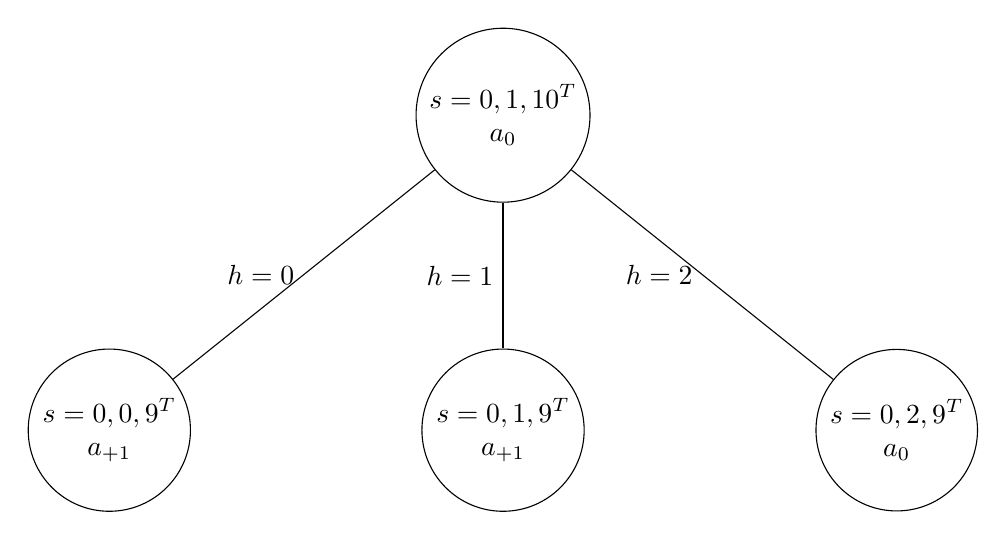
\begin{tikzpicture}
        \node[vertex_style](a) at (0,0) {
          $s = \br{0, 1, 10}^T$ \\
          $a_0$
        };
        \node[vertex_style](b) at (-5,-4) {
          $s = \br{0, 0, 9}^T$ \\
          $a_{+1}$
        };
        \node[vertex_style](c) at (0,-4) {
          $s = \br{0, 1, 9}^T$ \\
          $a_{+1}$
        };
        \node[vertex_style](d) at (5,-4) {
          $s = \br{0, 2, 9}^T$ \\
          $a_{0}$
        };
        \draw (a)--node[left]{$h=0$}(b);
        \draw (a)--node[left]{$h=1$}(c);
        \draw (a)--node[left]{$h=2$}(d);
      \end{tikzpicture}
    \end{center}

  \item[\#11]
    If we are using the fast informed bound (FIB) to approximate the optimal
    value function, how many alpha vectors will there be?

  \item[\#12]
    If $\alpha_{QMDP}$ is an alpha vector generated by QMDP and $\alpha_{FIB}$
    is an alpha vector generated by FIB, can there exist a $b$ such that
    $b^T \alpha_{QMDP} \le b^T \alpha_{FIB}$?
    Why or why not?

  \item[\#13]
    Suppose we have a belief state $b$ that assigned probability $0.5$ to
    $\br{0, 0, 1}^T$ and probability $0.5$ to $\br{1, 0, 1}^T$.
    What is the value for $U^*(b)$ in terms of $\lambda$ (which may take on any
    negative value)?

  \item[\#14] % Done
    Why would you not use a particle filter to update your belief for this
    problem?

    You would not use a particle filter to update your belief for this problem,
    because the state space is not particularly large or continuous.
    A particle filter is sampling approach that uses particle to sample the
    state space.
    In this case the state space is small enough to be enumerated and so
    sampling isn't necessary.

  \item[\#15]
    Suppose your initial belief is uniform over the state space and then you
    observe that aircraft $A$ is $3$ units above aircraft $b$ after executing
    $a_0$.
    What probability would an exact Bayesian update of your belief state assign to
    aircraft $B$ being non-responsive?
    Why?

  \item[\#16]
    Write a little paragraph about what you learned in this class.
\end{enumerate}
\end{document}

